\section{Afforestation and Reforestation}
Afforestation and reforestation were modeled based on the available land, the amount of biomass that can be stored on these lands based on the climate zones, and the carbon content of said biomass. Two scenarios are considered: a natural (assisted) regeneration approach, which is a low-intervention process that fosters natural forest regrowth only by removing weeds and preventing soil degradation, and forest plantations through manual planting.

\subsection{Land availability}
To estimate the available land, data on the land area deforested worldwide since the year 2001 was collected from Global Forest Watch \parencite{world_resource_institute_forest_2025}. This cutoff was used to create a sufficiently conservative estimate of areas that could be reforested, considering the expansion of human settlements, industrial areas, and other infrastructure that displaced forests earlier on and cannot realistically be reforested. The land availability data was then combined with data on climate zones based on high-resolution Köppen-Geiger climate maps by \textcite{beck_high-resolution_2023}. The open-source QGIS application was used to calculate numerical average climate values for each country, which were then converted back to the Köppen-Geiger scale using the mapping from \textcite{beck_high-resolution_2023}. Finally, all "A" climate zones were labeled as tropical, the "B" and "C" climate zones as temperate, the "D" zones as boreal and the "E" zones as arctic. Only tropical, temperate and boreal zones were considered for afforestation.\vspace{2mm}

\begin{wrapfigure}{l}{0.6\textwidth}
\vspace*{-7mm}
%\setlength{\columnsep}{0pt}
  \centering
  \small
    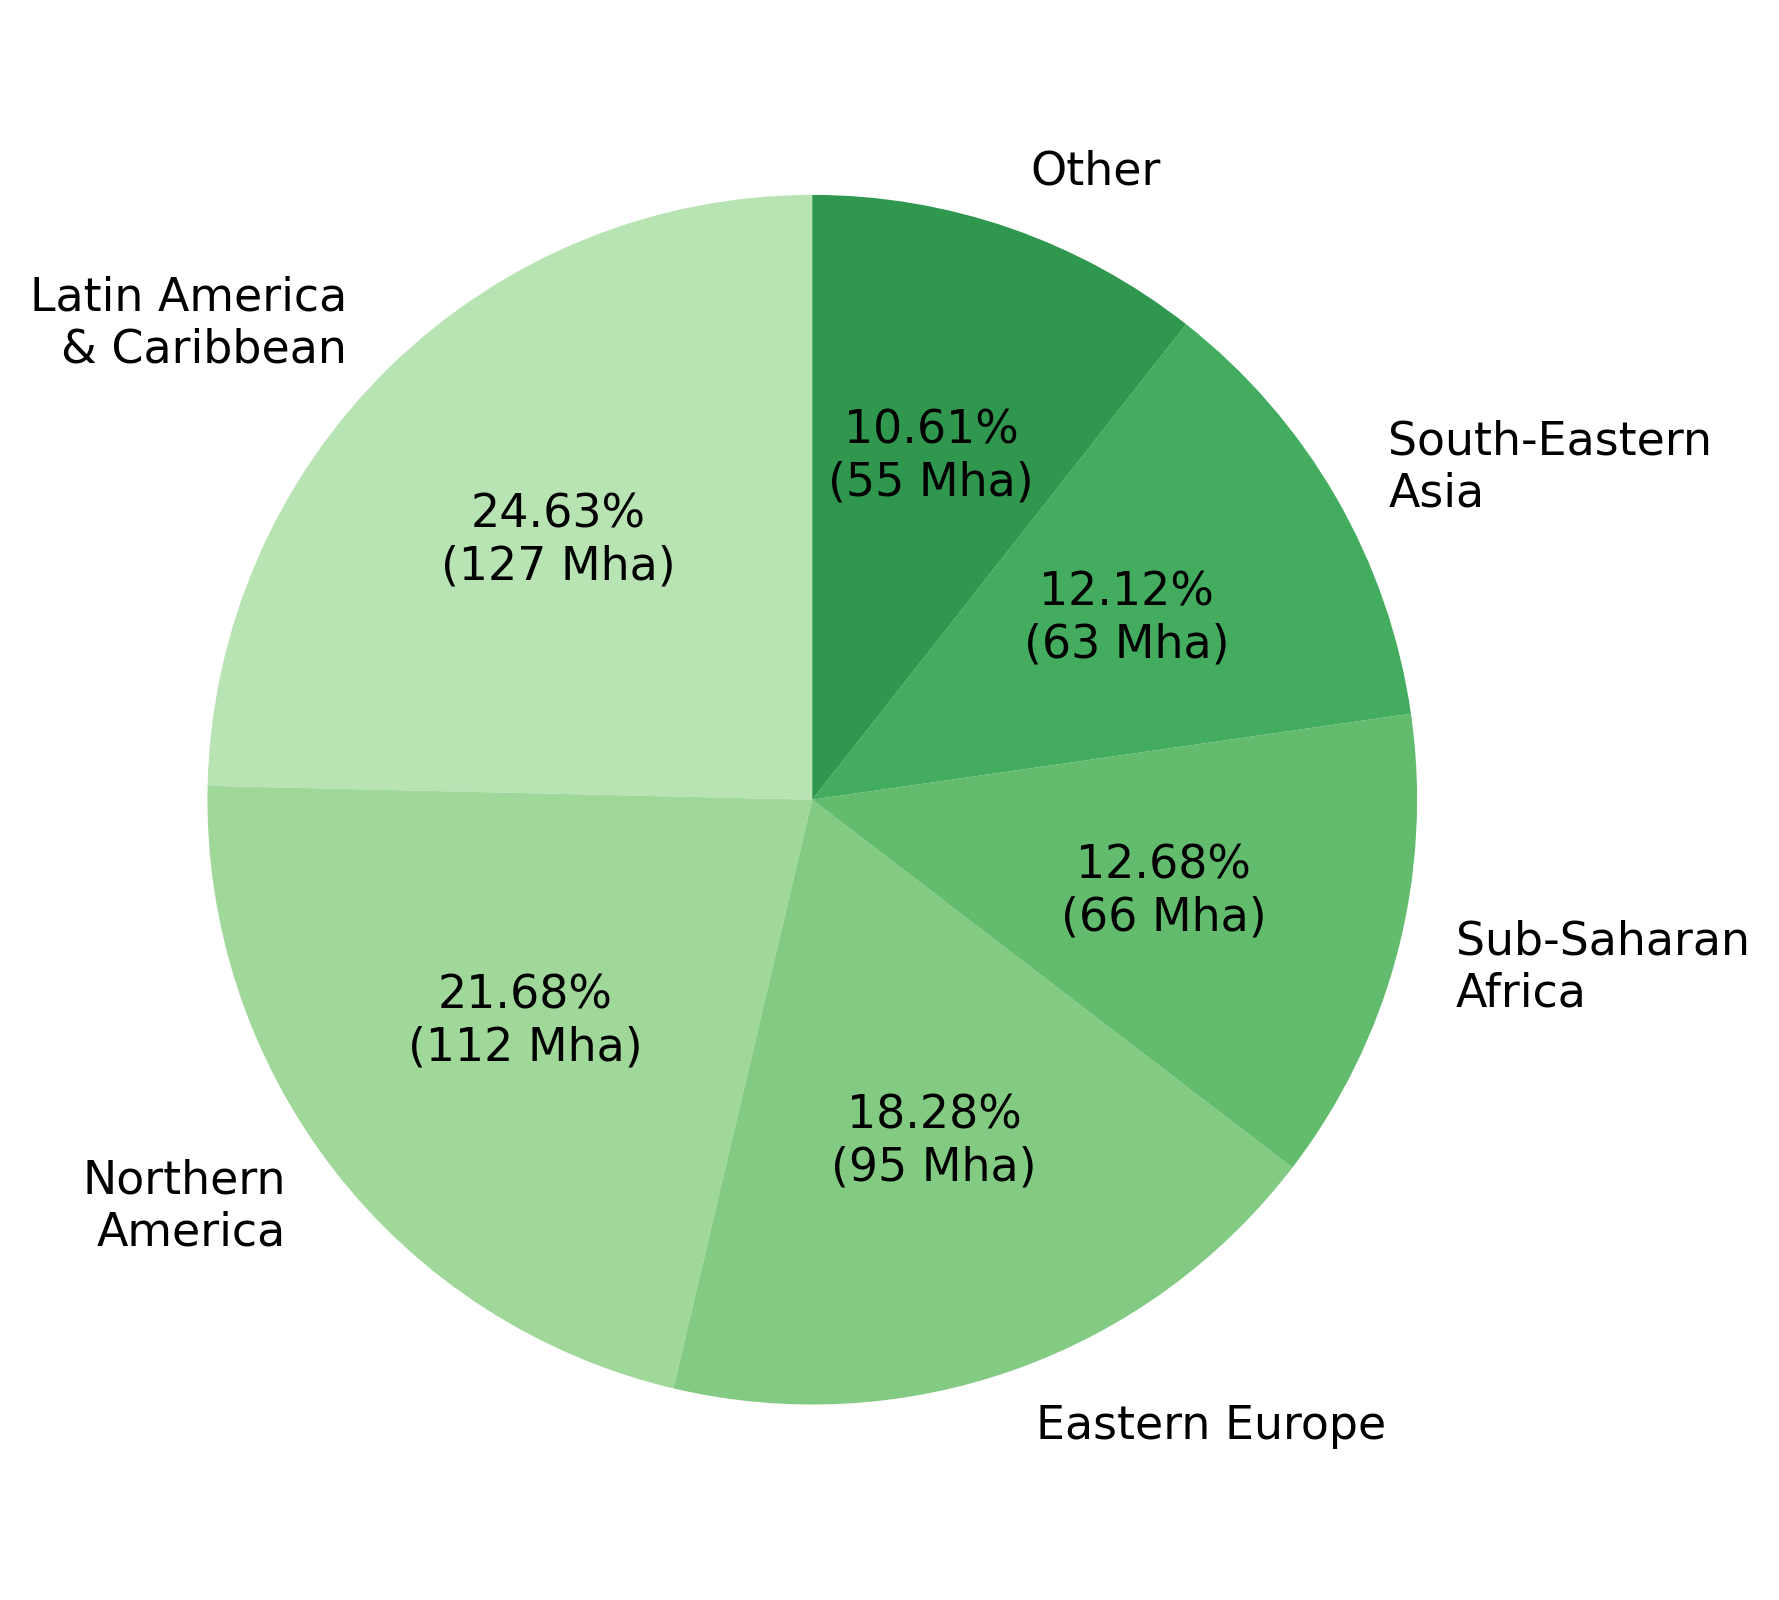
\includegraphics[width=0.58\textwidth]{figures/total_tree_cover_loss_by_continent.png}
    \caption{Global tree cover loss since 2001, by region}
%\vspace*{-\baselineskip}
\end{wrapfigure}

To calculate the annual A/R-based carbon removal potential by country, the annual biomass growth rates and total biomass accumulation per hectare were collected from the "2006 IPCC Guidelines for National Greenhouse Gas Inventories" \parencite{eggleston_2006_2006}. This allowed for the calculation of the growth years and, using an estimated carbon content of 50\% and the CO$_2$-to-C ratio of 44/12, the annual CO$_2$ uptake per hectare of new forest. Additionally, an annual loss of stored carbon of 1\% was included to account for reversal.

\subsection{Assisted natural regeneration}
Assisted natural regeneration is a relatively cheap process which increases the productivity of degraded lands by facilitating the natural regrowth processes. It typically results in a diverse and sustainable ecosystem, requires little infrastructure and capital investments, and is therefore suitable for deployment even in poor or hard-to-access regions with little available infrastructure. The only manual labour used is typically the removal of invasive species and other undesired weeds. However, assisted natural regeneration requires natural seeding, which means that it can only work if at least some forest areas are present nearby \parencite{busch_cost-effectiveness_2024, crouzeilles_achieving_2020, chazdon_natural_2016}.\vspace{2mm}

\begin{figure}[ht]
  \begin{center}
    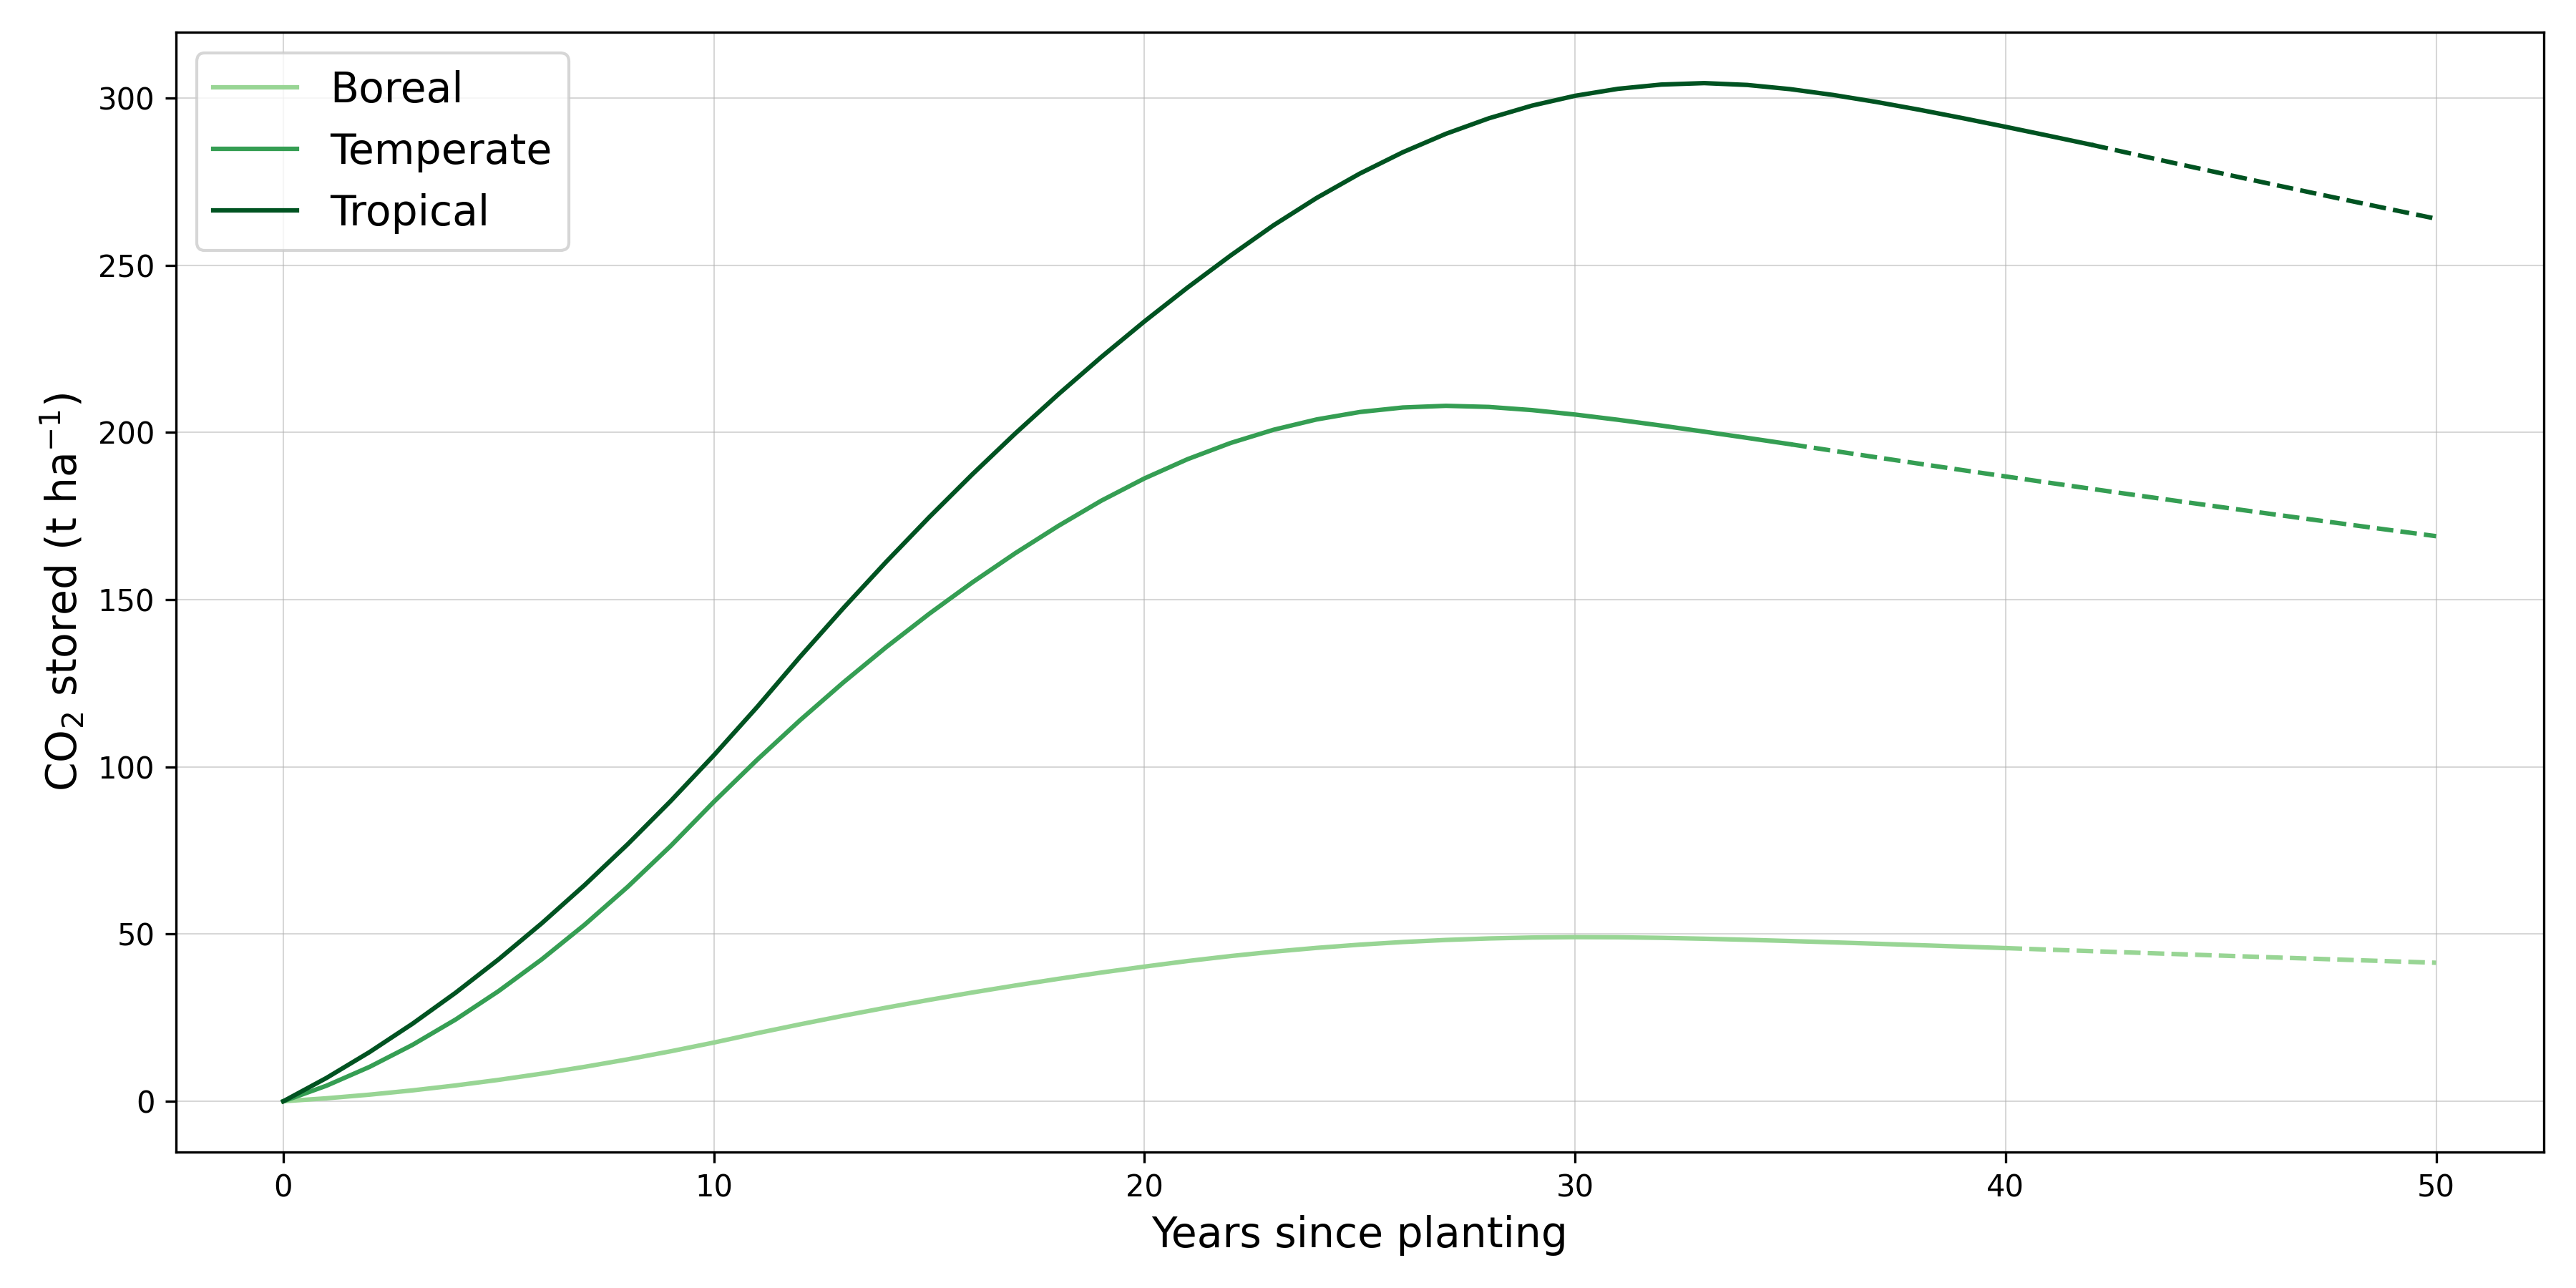
\includegraphics[width=1\linewidth]{figures/forest_cycle.png}
    \caption{Forest growth cycles in various climate zones - assisted natural regeneration}
    \label{fig:forest_cycle}
  \end{center}
  %\vspace*{-\baselineskip}
\end{figure}

The growth cycle of a forest restored using assisted natural regeneration is shown in figure 3.2. Depending on the climate zone, the growth cycle lasts between 35 and 42 years, after which the maximum biomass density is achieved in trees that have survived until that point. The decline in stored carbon, which begins already before the end of the growth phase, is explained by the reversal, which exceeds the accumulation of carbon from additional growth during the late stages of the growth phase. At the peak, tropic rain forests store over 300 tonnes of CO$_2$ per hectare, while forests in temperate zones store over 200 tonnes of CO$_2$ and boreal forests only reach about 50 tonnes of CO$_2$ per hectare.


\subsection{Forest plantations}
In forest plantations, forests are purposely planted either for commercial use or for forest restoration. The primary difference between the two types is that commercial forest plantations often consist of mono-cultures of a single species intended for harvesting, while forests planted for restoration are more diverse and intended to result in a sustainable ecosystem. However, this also means that the latter can be significantly more expensive, costing over 10.000 USD per hectare just for establishment, compared to around 4.000 USD per hectare for commercial-use forest plantations \parencite{bodin_standard_2022}. The primary advantage of forest plantations is the faster growth resulting from manual planting, as shown in figure 3.3.

\begin{figure}[ht]
  \begin{center}
    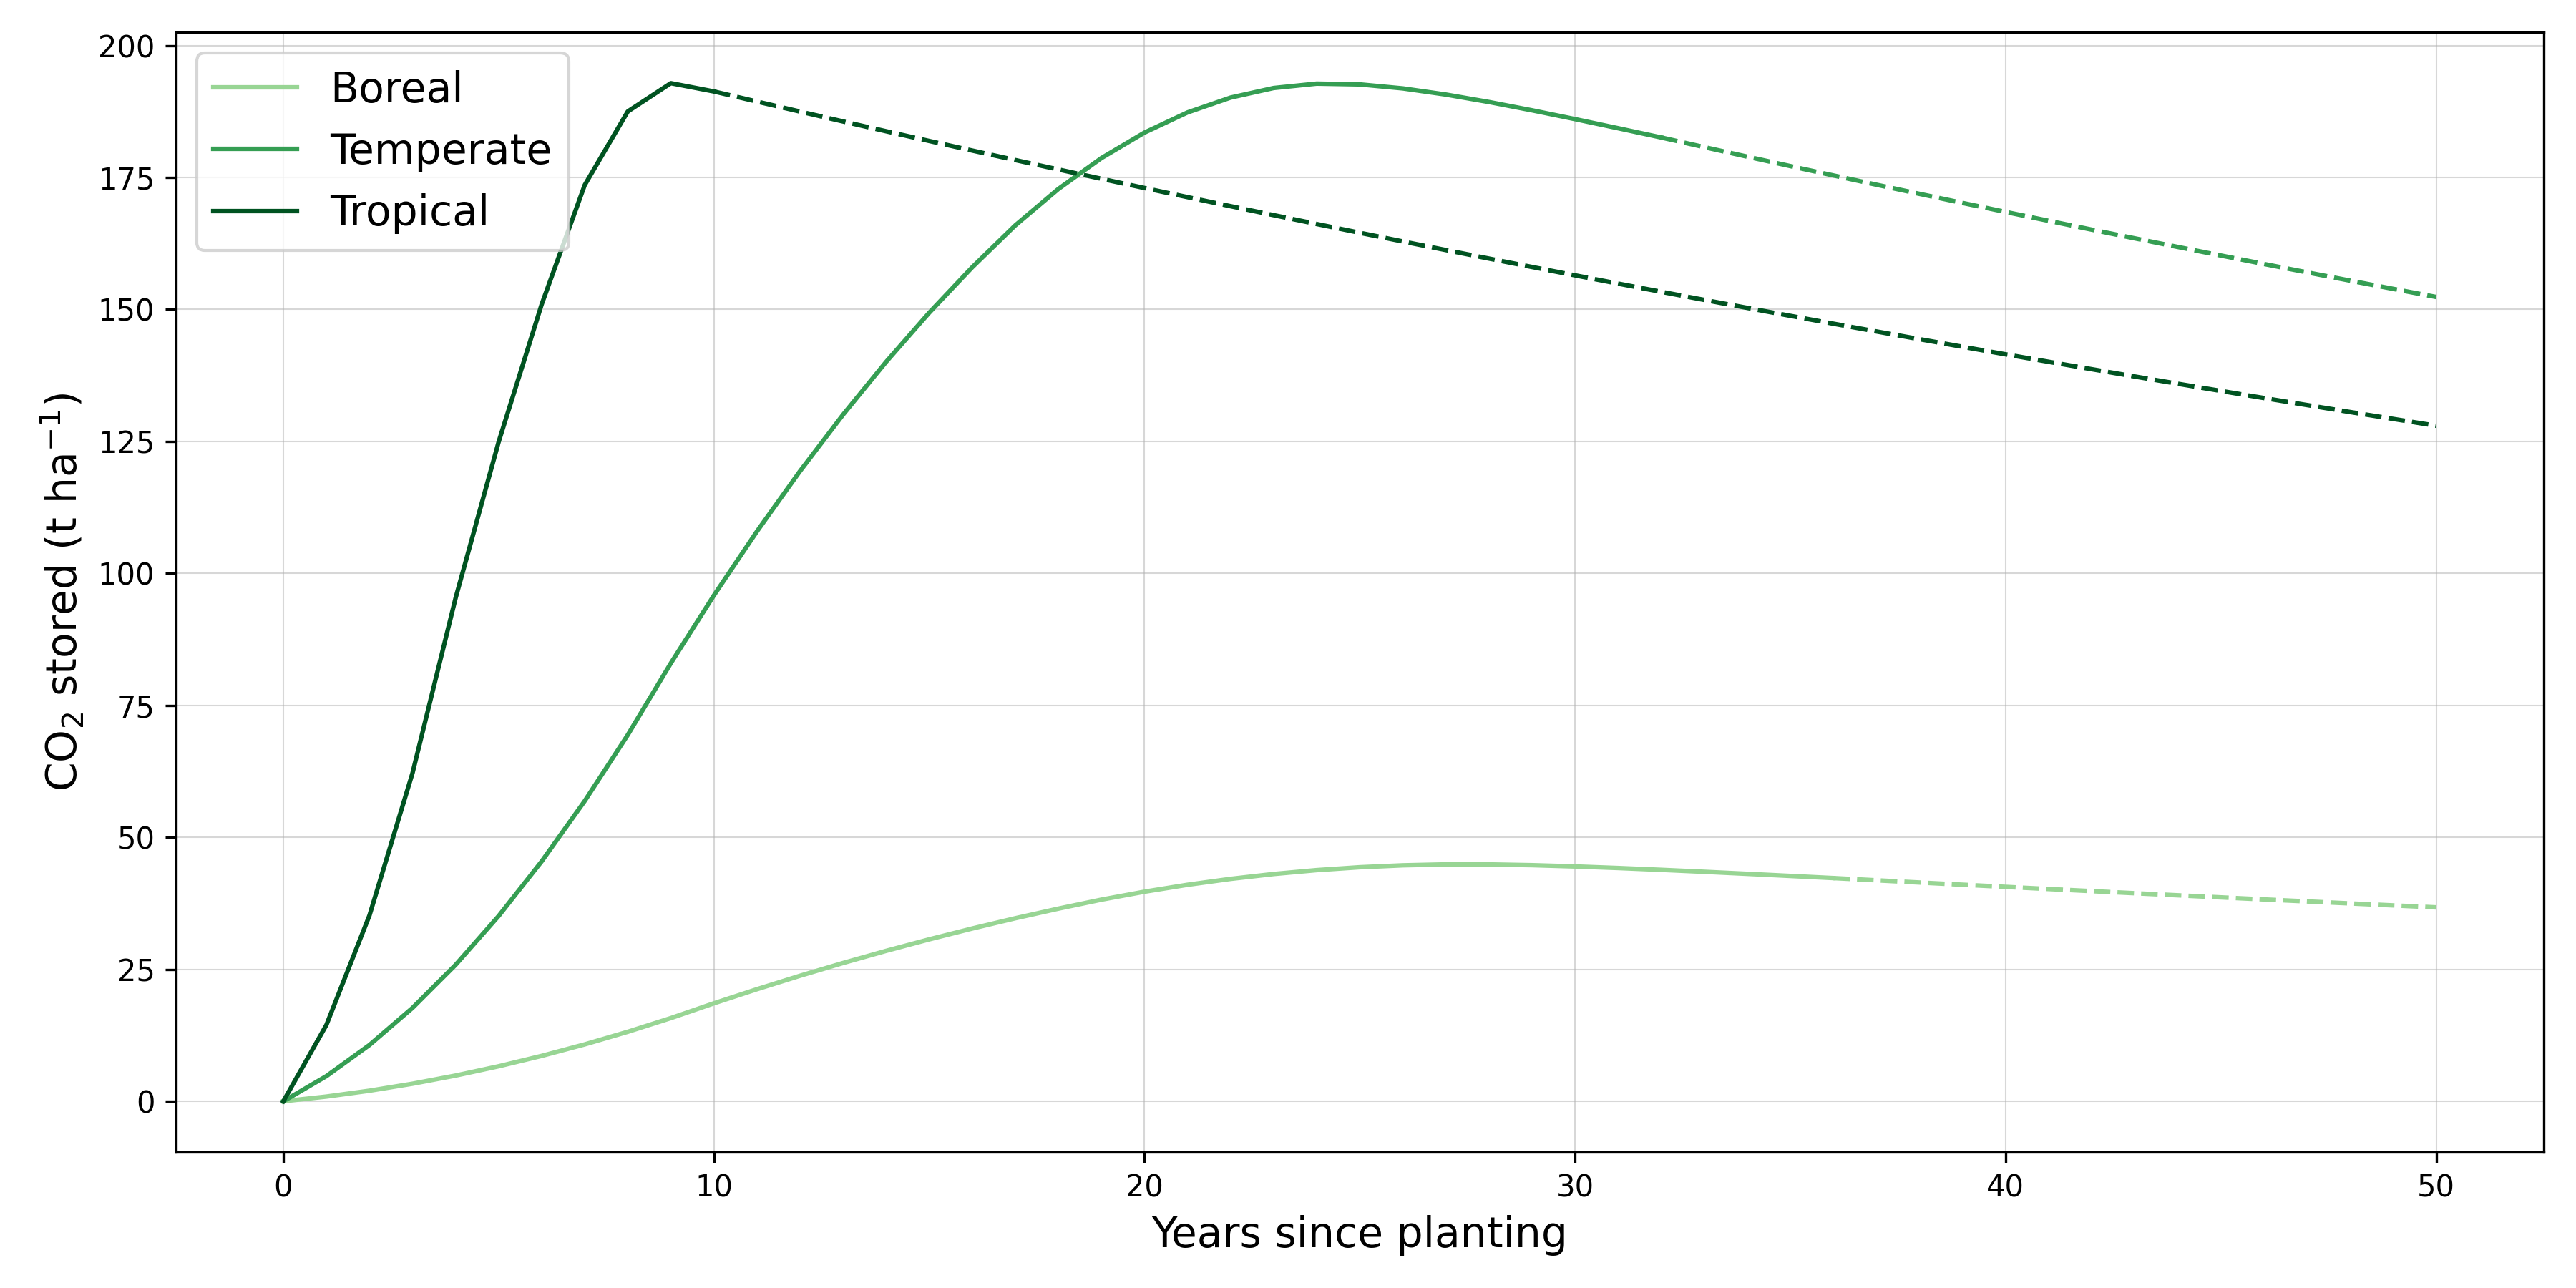
\includegraphics[width=1\linewidth]{figures/forest_cycle_plantation.png}
    \caption{Forest growth cycles in various climate zones - forest plantation}
    \label{fig:forest_cycle}
  \end{center}
  \vspace*{-\baselineskip}
\end{figure}

\subsection{Cost modeling}

To model the cost of afforestation and reforestation, two components were considered: The cost of establishing the new forests as the capital investment, and the cost of maintenance as the annual fixed cost. The opportunity cost, that is, the foregone profits from using the afforested lands in other capacities, was not considered. In order to develop reasonable cost estimates, previous research by \textcite{bodin_standard_2022} and \textcite{forbes_review_2022} was used to calculate average values for the establishment and maintenance of both, assisted natural regeneration forests and forest plantations. For the maintenance cost, it was assumed that 10 years of active efforts are required, and a present value formula using a discount rate of 7\% was applied to calculate the total cost of maintenance. Finally, and similar to the other NET models, a PPP factor was applied to adjust the cost for each country. The resulting marginal abatement cost curves for both approaches are shown in figures 3.4 and 3.5.\vspace{2mm}

\begin{figure}[ht]
  \begin{center}
    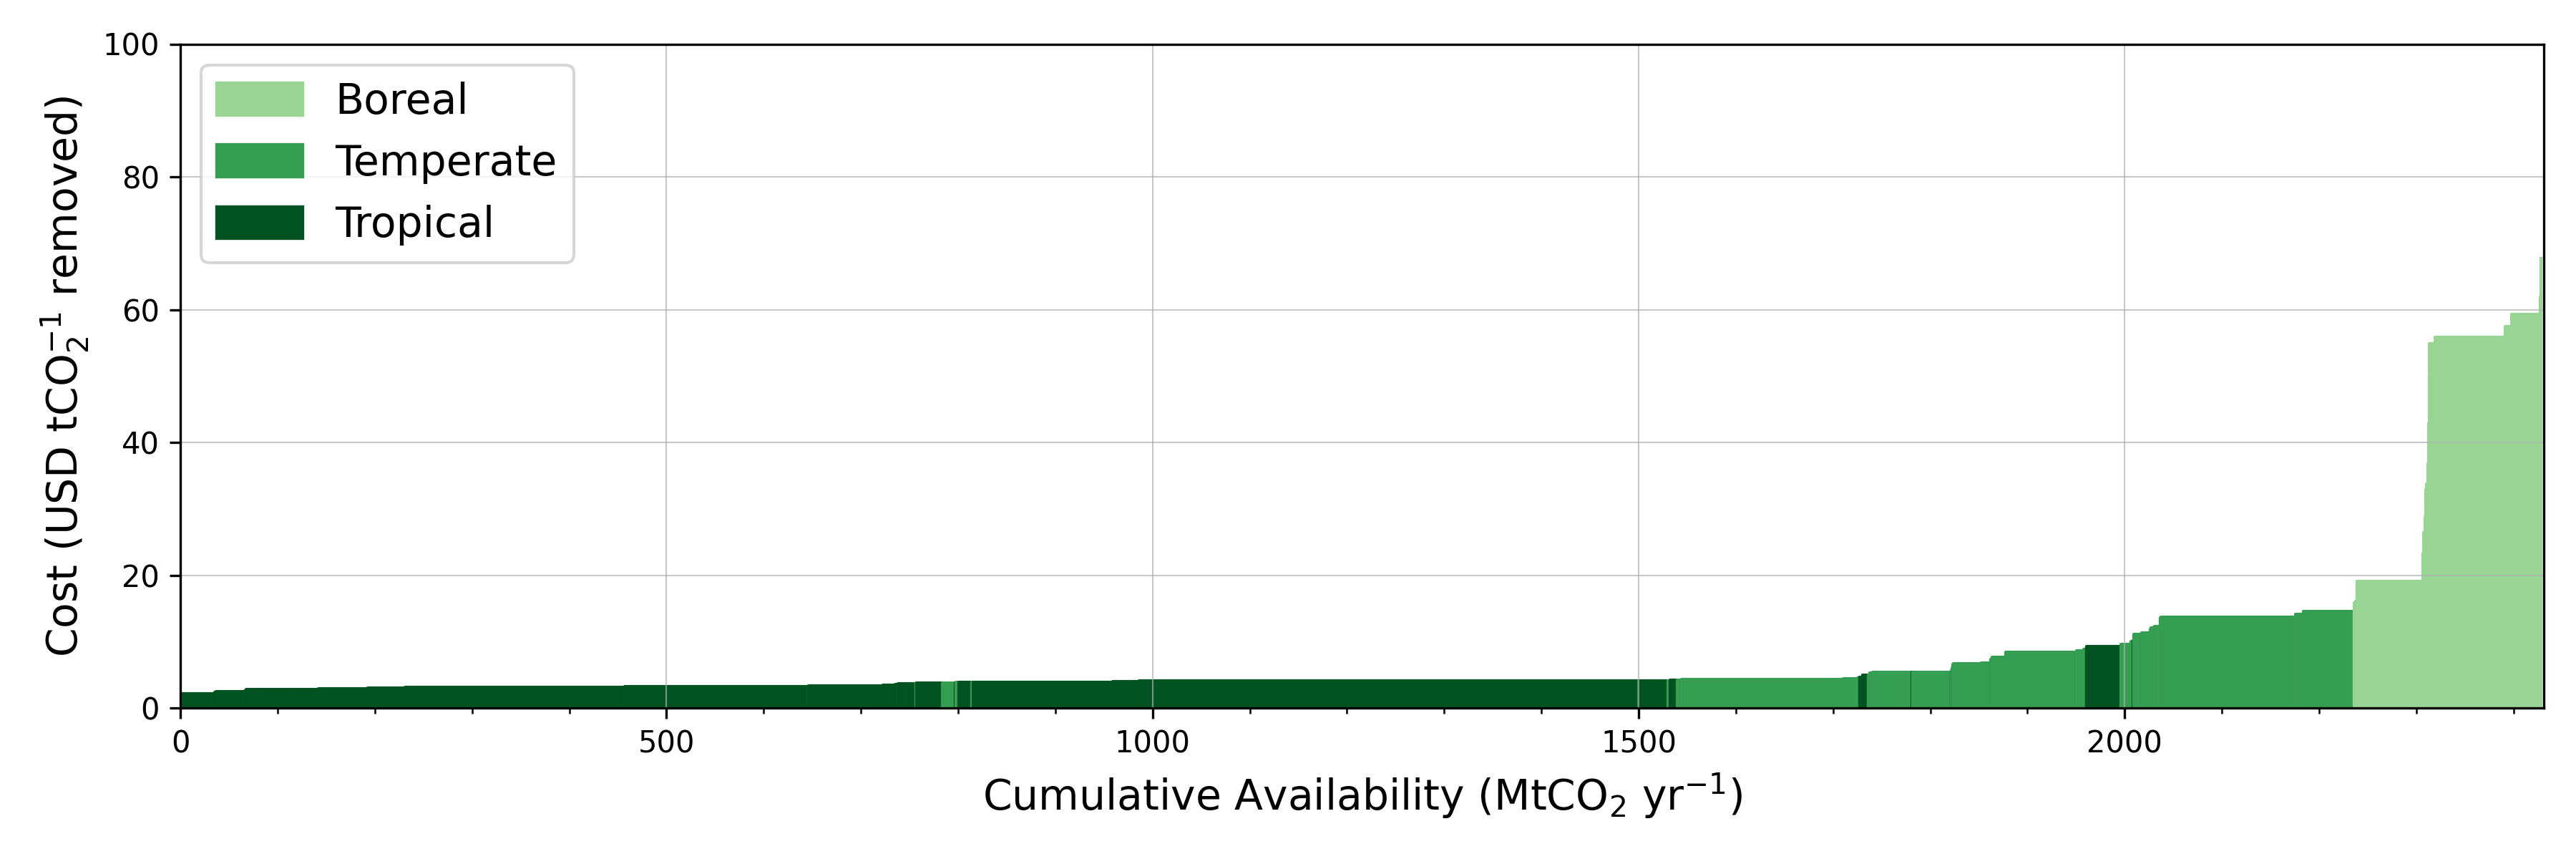
\includegraphics[width=1\linewidth]{figures/afrf_macc_chart.png}
    \caption{Global Afforestation marginal abatement cost curve - assisted natural regeneration}
    \label{fig:forest_cycle}
  \end{center}
  \vspace*{-\baselineskip}
\end{figure}
\newpage

If assisted natural regeneration is used, the majority of the global annual potential of about 2.5 GtCO$_2$ is available at an LCOC$^+$ below 10 USD tCO$_2^{-1}$, with the remainder of the tropical and temperate regions coming in at below 20 USD tCO$_2^{-1}$. The boreal forest-based CDR is significantly more expensive due to the much lower overall biomass accumulation per hectare in these regions, but still costs less than 80 USD tCO$_2^{-1}$.\vspace{2mm}

\begin{figure}[ht]
  \begin{center}
    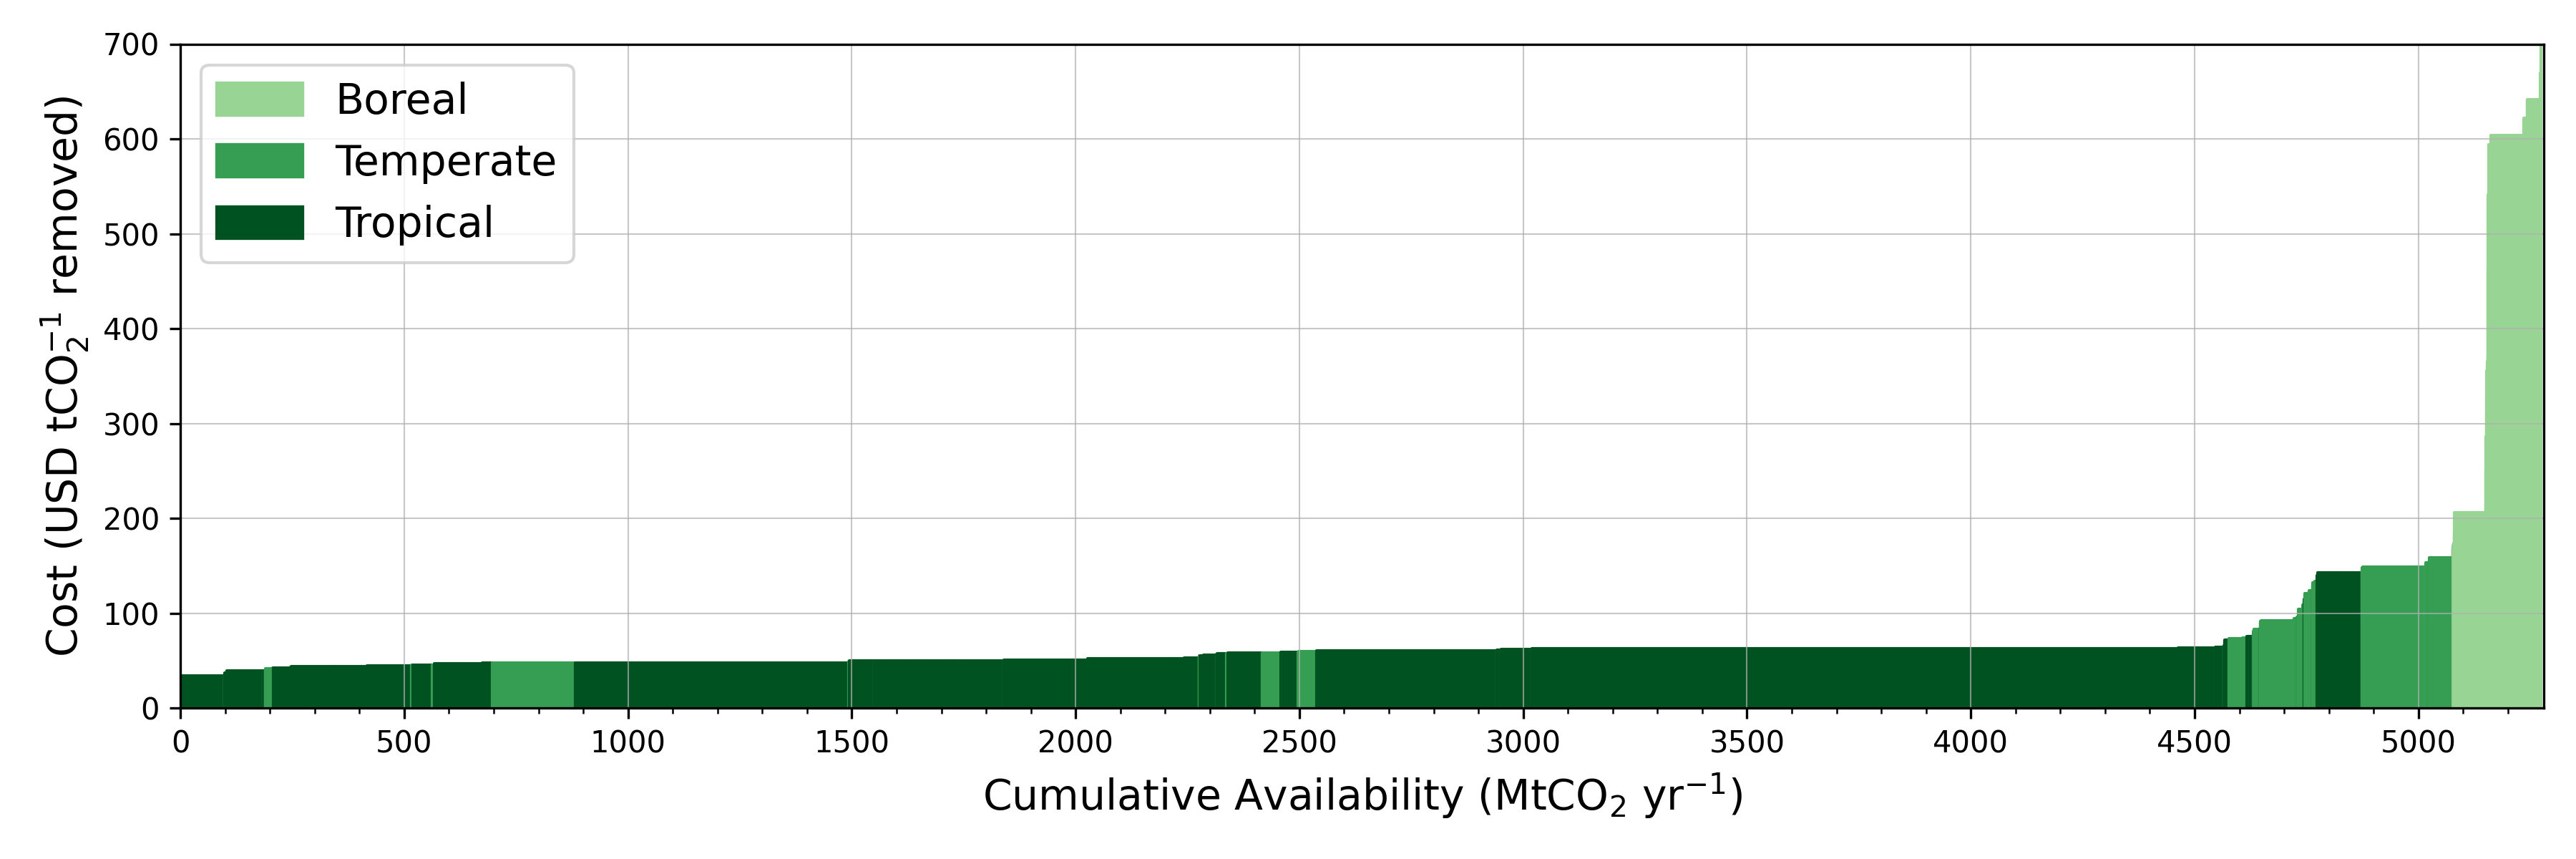
\includegraphics[width=1\linewidth]{figures/afrf_macc_chart_plantation.png}
    \caption{Global Afforestation marginal abatement cost curve - forest plantation}
    \label{fig:forest_cycle}
  \end{center}
  \vspace*{-\baselineskip}
\end{figure}

In comparison, using forest plantations is considerably more expensive, primarily due to the use of saplings and the labor required to plant them. The study by \textcite{forbes_review_2022}, concerning A/R in New Zealand, estimates that over 4000 saplings are used per hectare, requiring more than 270 hours of labor to plant and maintain. Consequently, the majority of forest plantation-based CDR is available at around 60 USD tCO$_2^{-1}$, while costs in boreal regions can reach over 600 USD tCO$_2^{-1}$. The global annual CDR potential using forest plantations is significantly higher than that of assisted natural regeneration, at around 5.5 GtCO$_2$ yr$^{-1}$, owed to the much faster growth of trees. However, it should be noted that this does not increase the available amount of land or biomass accumulation per hectare. Instead, the available land is used faster, and the overall CDR potential exhausted earlier. Also note that these results are considered an LCOC$^+$ because maintenance costs, and therefore the potential cost of reversals, are included in the model.\vspace{2mm}

\subsection{Risk and permanence}

Compared to the other NETs considered in this thesis, A/R faces the fundamental issue of lacking permanence. While geologic carbon storage, whether in the form of concentrated CO$_2$ or mineralized solutions, can be expected to last for many centuries and even millennia with little leakage, forests are at a much higher risk of reversal due to fires, pests or human intervention \parencite{smith_state_2024}. While this clearly creates doubt about whether A/R should even be considered compared to the other NETs, many carbon reduction and removal pathways, such as \textcite{mulligan_carbonshot_2020}, involve significant amounts of A/R and other land and forestry-based approaches. Considering the amount of CDR required and the currently lacking progress of both, emission reductions and removals, not considering A/R would be unreasonable. Instead, it is important to remain conscious of these differences in permanence and properly account for them. In the optimization model constructed later in this thesis, an assumed 1\% annual reversal rate, which simulates the release of stored carbon to the atmosphere and frees the respective land area for another cycle of afforestation, is added to make the results more comparable to these of the other NETs.
